
\chapter{Описание прототипа}
%\label{cha:prorotype_description}
В описании авторского свидетельства № 1725070 МПК G01B 7/00 (по заявке № 4822394/28 от 22.03.90 г., автор В. Г. Панов) \cite{patent} представлено устройство «Ёмкосный датчик микроперемещений». Эскиз которого представлен на рисунке \ref{fig:draw}

\begin{figure}[]
    \centering
    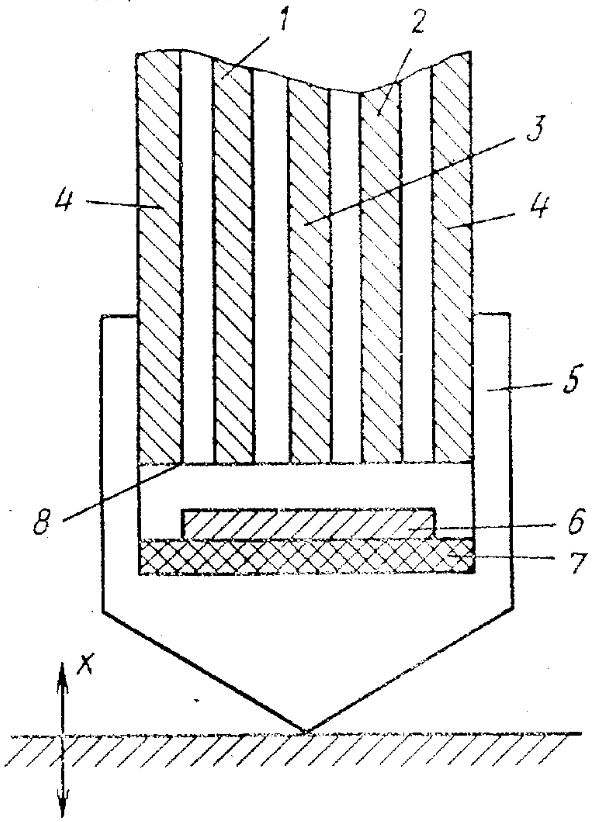
\includegraphics[width=0.7\textwidth]{graphics/img/draw.png}
    \caption{Эскиз прототипа}
    \label{fig:draw}
\end{figure}

Датчик содержит неподвижно закрепленные в корпусе потенциальный стержневой электрод 1 и установленный параллельно ему измерительный электрод 2, который отделен от потенциального электрода внутренним стержневым экраном 3. Внешний экран 4, выполненный в виде полого цилиндра, охватывает электроды датчика. Снаружи боковой цилиндрической поверхности внешнего экрана 4 размещен с возможностью возвратно-поступательного движения щуп 5, во внутренней полости которого размещена тонкая металлическая пластина 6, электрически изолированная от корпуса датчика с помощью диэлектрической прокладки 7 и расположенная параллельно рабочей плоскости 8 электродов и экранов датчика. Щуп 5 датчика упирается в поверхность контролируемого объекта, перемещение которого измеряется. 

Датчик работает следующим образом. При перемещении объекта изменяется воздушный зазор между плоскостью металлической пластинки 5 и рабочей плоскостью 8 электродов 1 и 2 и экранов 3 и 4 датчика, вследствие чего изменяется выходное напряжение $U_{\text{вых}}$ снимаемое с измерительного электрода 2 датчика. Чувствительность датчика зависит от величины диэлектрической постоянной материала контролируемого объекта и максимальна в диапазоне $[0 : x_{\text{мин}}]$, где $x$ - величина микроперемещения, когда металлическая пластина 6 не заземлена. Герметизация щупа 5 позволяет свести к минимуму погрешности, связанные с влиянием внешних условий.

\chapter{Анализ и синтез систем}
\label{cha:analis0}

\section{Анализ и синтез по закону полноты частей системы}

Полную ТС можно представить в виде структурной схемы, как показано на рисунке \ref{fig:analysis1_example}, где ЕЭ - источник энергии, а Изд. - изделие. Ро - рабочий орган, Тр - подводит энергию к Ро от Дв. (трансмиссия), Дв. - вырабатывает энергию, Оу - управляет работой всех или хотя бы одной частью системы. \cite{metodichka}

\begin{figure}
    \centering
    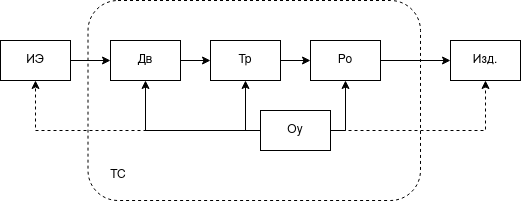
\includegraphics[width=0.8\textwidth]{graphics/img/analys1_example.png}
    \caption{Структурная схема полной технической системы}
    \label{fig:analysis1_example}
\end{figure}

Для описания по законы полноты частей системы следует определить основные функциональные элементы, представленные на рисунке \ref{fig:draw} соответствующие структурной схеме на рисунке \ref{fig:analysis1_example}.

Источником энергии в данной системе служит внешний источник питания, который подаёт питающее напряжение на потенциальный электрод и даёт ему положительный заряд.

Трансмиссией в данной системе служит потенциальный электрод 1. Преобразующий энергию в электромагнитное поле конденсатора между пластинами 1 и 6

Рабочим органом, органом управления, а также двигателем является щуп 5. Так как он непосредственно взаимодействует с измеряемой поверхностью перемещаясь перпендикулярно оси измеряемой плоскости. Щуп 5 приводится в движение за счёт давления оказанного от измеряемой плоскости. За счёт изменения воздушного зазора между электродами 1 и 6 изменяется и диэлектрическое сопротивление между ними, следовательно щуп 5 является и органом управления.

\section{Анализ и синтез по закону энергетической и информационной проводимости ТС}

Необходимым условием для принципиальной жизнеспособности ТС является сквозной проход энергии и информации по всем частям ТС. В соответствии с этим утверждением на рисунке \ref{fig:process} представлена линия прохода энергии/информации в анализируемой ТС.

\begin{figure}
    \centering
    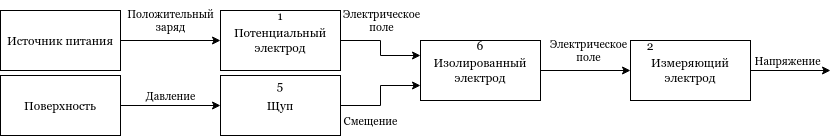
\includegraphics[width=\textwidth]{graphics/img/process_scheme.png}
    \caption{Линия прохода энергии/информации}
    \label{fig:process}
\end{figure}

Анализируя представленную схему можно заключить, что система разделяется на механическую (от поверхности производящее давление на щуп до измерительного электрода) и электрическую (от потенциального электрода, заряженного от внешнего источника питания к измерительному электроду) потоки энергии, где сводятся в один поток выдавая на выходе напряжение $U_{\text{вых}}$ соответствующая разности потенциалов между 1 и 2 электродами.

\section{Закон согласования-рассогласования технических систем}

